\section{Introduction}
\subsection{Background}
\subsubsection{Stewart Platform}
\subparagraph*{Description of Mechanism}
\paragraph{}A stewart platform is a platform with six degrees of freedom (DOF). The six-degrees-of-motion platform is capable of moving in three linear directions and
three angular directions singly or in any combination.
It comprises a triangular/rectangular/circular plane called the platform, of which each of the corners (for triangualar platform in this case) is connected through a three-axis joint to one of three legs. This is shown in Fig.1.1.
\begin{figure}[!h]
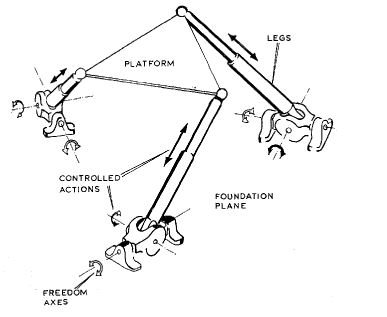
\includegraphics{Figures/Fig1}
\caption{General arrangement}
\end{figure}
\paragraph{}Each leg is connected to the ground by a two-axis joint where: One of these axes is
normal to the leg and is provided with a means for control wheareas, the other axis is normal to the first and is not provided with a means for control.
Each leg also has controllable means for extending its length. These control means include:
\begin{enumerate}
\item Use of two hydraulic jacks
\item Screw Jacks
\item Rotary actuator
\item Levers
\item Linear co-ordinate control
\item Strength
\end{enumerate}
\paragraph{}These shall be discussed in detail at a later stage.

\subparagraph{Application}
\paragraph{}The six DOF Stewart Platform provides an elegant design for simulating flight conditions which finds applications in the safe training of pilots. The mechanism differs from other simulators in that it has no fixed axes relative to the ground, and therefore within the limits of amplitude of the design it can truly simulate the conditions of banking by carrying the simulation of control surfaces into the axes of the new attitude.

\subsubsection{Force Balance}
\subsubsection{Wind Tunnel}
\paragraph{}
A wind tunnel is a large tube with air moving inside. This movement of air is usually done by powerful fans. The tunnel is used to copy the actions of an object in flight. The first wind tunnel was built by
Francis Wenham in 1871. However, it was the Wright Brothers who were the first to show the value of the wind tunnel in aerodynamic design with their 1902 wind tunnel.  The Wright Brothers’ wind tunnel was largely made of wood, with a glass window on the top to look down through and see the force balance, from which the
lift and drag forces could be read. The wind tunnel was powered by a fan driven off a natural gas fueled engine. Their tunnel was square of 16" by 16"(about 407mm by 407mm), and 6 foot long (about 1829mm), with a maximum test speed of 35 mph (about 56 km/h).
\begin{figure}[!h]
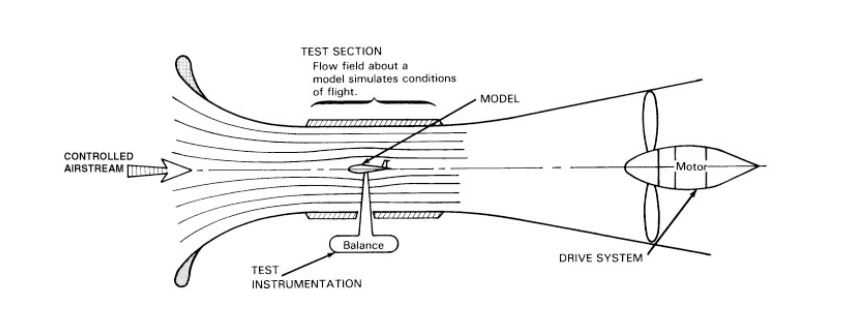
\includegraphics{Figures/Fig2}
\caption{Diagram of a typical wind tunnel}
\end{figure}
\paragraph{}
Later in the early 20th century in Europe, the main users of wind tunnels were Gustave Eiffel in France and Ludwig Prandtl in Germany. Prandtl built the first closed circuit wind tunnel in 1908. By the 1940’s supersonic wind tunnels were in use. In 1972 a cryogenic wind tunnel was built at NASA Langley by injecting liquid nitrogen into the wind tunnel to cool the gas. This lowered the viscosity and increased the Reynolds number, and this tunnel had the capability to match Reynolds and Mach numbers simultaneously up to Mach 1.2. 
\paragraph{}Today the largest wind tunnel in the world is the National Full-Scale Aerodynamics Complex at NASA's Ames Research Center, which has a test section of cross section 80 ft by 100 ft (24 m x 31 m). The types of instruments in common use in wind tunnels include boundary layer rakes, tufts, pitot tubes, pressure sensitive paint, smoke, and static pressure taps.
\begin{figure}[!h]
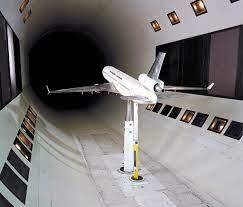
\includegraphics{Figures/Fig3}
\caption{NASA wind tunnels used to test new airplane designs}
\end{figure}

\paragraph{}NASA uses wind tunnels to test scale models of aircraft and spacecraft. Wind tunnels help NASA to test ideas of making airplanes better and safer. They are also used to help engineers in designing spacecraft that will work in other planets such as mars - the wind tunnel can be used to simulate objects in an atmosphere that's thinner than ours i.e. an atmosphere that's exactly like the Martian atmosphere. NASA has wind tunnels of different types and sizes. Some are low-speed wind tunnels, others are hypersonic i.e. they are made to carry out tests at 4,000 mph (6437 kph).
\begin{figure}[!h]
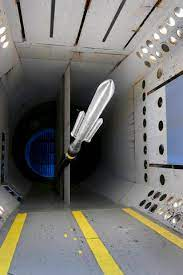
\includegraphics{Figures/Fig4}
\caption{NASA wind tunnels used to test the design of heavy-lift rocket}
\end{figure}
\paragraph{}Wind tunnels are used to measure the aerodynamic forces on airplanes, wings, cars, trucks, bridges, and buildings, they can also be used to measure the
aerodynamic forces on sports balls, partially open valves, and anything else that can be mounted on the mounting sting. Wind tunnels are an effective tool used by engineers in determining the various aerodynamic loads due to movement of these vessels during the development process.
For wind tunnel testing with scale models to be applicable to the aerodynamics of the full-scale test object, conditions of dynamic similarity must be met.
\paragraph{}Wind tunnel testing is not cheap i.e. both to buid and to use. While a crude wind tunnel can be constructed relatively cheaply from a large fan and
sheet metal, our project will be limited to development of the six-degrees-of-freedom Stewart Platform and Force balance. We will use the low speed wind tunnel that is currently available at ?????
\subsection{Problem statement}
(Insert your content)
\subsection{Objectives}
\cite{stewart_platform_1965}
\subsection{Justification of the study}
\paragraph{}Additive manufacturing offers the ability to produce intricate products and parts with lower development costs, shorter lead times, less energy consumed during manufacturing as well as less material waste. This method can be used to manufacture delicate components such as the bipolar plates with elimination of the risks involved such as breakage of brittle Graphene material during production.     
\paragraph{}Precise control of reactant flow and pressure, stack temperature, and membrane humidity will increase the fuel cell’s robustness as well as efficiency.
\paragraph{}The goal of this research is to develop physic-based dynamic models of fuel cell systems and fuel processor systems and then apply multivariable control techniques to study their behavior. The analysis will give insight into the control design limitations and provide guidelines for the necessary controller structure and system re-design.
